% LaTeX
% vim: fen

\documentclass[12pt]{article}

\usepackage[a4paper, vmargin=10pt, hmargin=50pt, head=16pt, includehead]{geometry}
\usepackage{amsmath}     % math
\usepackage{amssymb}     % math symbols
\usepackage{enumitem}    % enumerate/list items
\usepackage{fancyhdr}    % header
\usepackage{mathtools}   % math tools
\usepackage{multicol}    % multiple columns
\usepackage{pgfplots}    % graphs
\usepackage{titlesec}    % alternative section titles
\usepackage{xcolor}      % color text

\usepgfplotslibrary{fillbetween}

\newcommand*\diff{\mathop{}\!\mathrm{d}}
\newcommand{\case}[1]{\textrm{#1$^\circ$}}
\newcommand{\degree}{^{\circ}}
\newcommand{\for}{\ \leftrightarrow\ }
\newcommand{\Integral}[4]{\int_{#1}^{#2} \! #3 \, \mathrm{d}#4}
\newcommand{\mathcolorbox}[2]{\colorbox{#1}{$\displaystyle #2$}}
\newcommand{\norm}[1]{\left\lVert#1\right\rVert}
\newcommand{\qed}{\textbf{\textit{QED}}}
\newcommand{\qef}{\textbf{\textit{QEF}}}
\newcommand{\task}[1]{\textbf{#1}}

\let\oldref\ref \renewcommand{\ref}[1]{\mathrm{(\oldref{#1})}}

\DeclareMathOperator{\?}{?}
\DeclareMathOperator{\dom}{dom}
\DeclareMathOperator{\im}{im}
\DeclareMathOperator{\lin}{lin}
\DeclareMathOperator{\R}{\mathbb{R}}
\DeclareMathOperator{\sgn}{sgn}

\let\oldepsilon\epsilon \renewcommand{\epsilon}{\varepsilon}

\counterwithin*{equation}{section}  % reset equation counter after each section
\titleformat{\section}{\normalfont\Large\bfseries}{}{0pt}{} % remove section numbering

\newcommand{\sectionbreak}{\clearpage} % start each section on new page

\setlength{\parskip}{0.7em}
\setlength{\parindent}{0em}

\pagestyle{fancy}
\lhead{Jakub Łukasiewicz}
\chead{Zestaw 14}
\let\Sectionmark\sectionmark
\def\sectionmark#1{\def\Sectionname{#1}\Sectionmark{#1}}
\rhead{\Sectionname}

\begin{document}
\section{Zadanie 1c}
Obliczyć pole obszaru ograniczonego podanymi krzywymi: $ y = 2^x, \quad y = 2, \quad x = 0 $

\subsection*{Rozwiązanie}

\begin{figure}[h!]
    \centering
    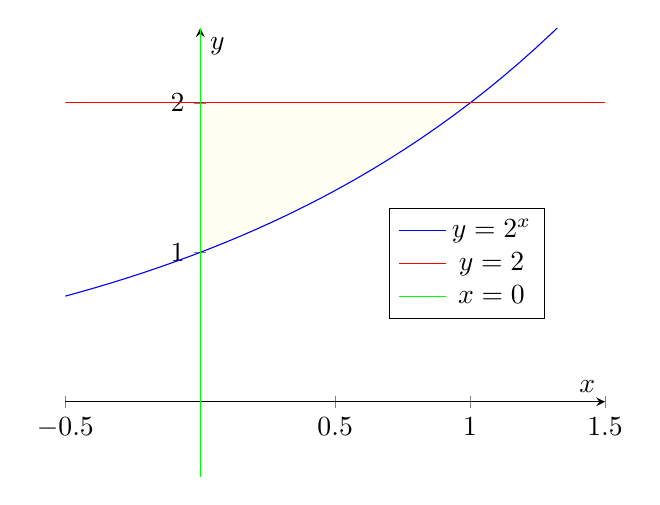
\begin{tikzpicture}[>=stealth]
        \begin{axis}[
                xmin=-0.5,xmax=1.5,
                ymin=-0.5,ymax=2.5,
                axis x line=middle,
                axis y line=middle,
                axis line style=->,
                xlabel={$x$},
                ylabel={$y$},
                legend style={at={(0.6,0.6)}, anchor=north west}]
            ]
            \addplot[blue] expression[domain=-3:3,samples=100]{2^x};
            \addplot[red] expression[domain=-3:3,samples=2]{2};
            \addplot[green] coordinates {(0, -1) (0, 3)};

            \addplot[name path=a, draw opacity=0,] expression[domain=0:1,samples=100]{2^x};
            \addplot[name path=b, draw opacity=0,] expression[domain=0:1,samples=2]{2};

            \addplot[fill=yellow, fill opacity=0.05] fill between[of=a and b];

            \legend{$y=2^x$, $y=2$, $x=0$}
        \end{axis}
    \end{tikzpicture}
\end{figure}

\begin{gather*}
    y = 2^x \implies x = \log_2{y} \\
    \because \textrm{ obszar jest na przedziale } [0,1]
\end{gather*}

\begin{equation*}
    S = \Integral{1}{2}{(\log_2{y})}{y} = \left[ \frac{x (\ln{x} - 1)}{\ln{2}} \right]_1^2 =
    \frac{2 (\ln{2} - 1)}{\ln{2}} - \frac{\ln{1} - 1}{\ln{2}} =
    2 - \frac{1}{\ln{2}}
\end{equation*}

\subsection*{Odpowiedź}
Pole tego obszaru wynosi $ \mathcolorbox{yellow}{2 - \frac{1}{\ln{2}}} $

\section{Zadanie 2a}

Obliczyć długość $L$ krzywej $ y = 2\sqrt{x^3} $, gdzie $ 0 \le x \le 11 $

\subsection*{Rozwiązanie}

\begin{equation*}
    (2\sqrt{x^3})' = 2(x^{\frac{3}{2}})' = 2 \cdot \frac{3}{2} \sqrt{x} = 3\sqrt{x}
\end{equation*}
\begin{equation*}
    L = \Integral{0}{11}{ \sqrt{1 + \left(3\sqrt{x} \right)^2 } }{x}
\end{equation*}
\begin{align*}
    \Integral{}{}{ \sqrt{1 + \left(3\sqrt{x} \right)^2 } }{x}
    &= \Integral{}{}{ \sqrt{1 + 9x } }{x} =
    \begin{vmatrix}
        \displaystyle t       = \sqrt{1 + 9x} \\[0.5em]
        \displaystyle \diff t = \frac{9}{2\sqrt{1+9x}} \diff x \\[1em]
        \displaystyle \diff x = \frac{2t}{9} \diff t
    \end{vmatrix}
    = \Integral{}{}{\frac{2 t^2}{9}}{t} =\\
    &= \frac{2}{9} \Integral{}{}{t^2}{t} =
    \frac{2t^3}{27} + C = \frac{2\left( \sqrt{1 + 9x} \right)^3}{27} + C
\end{align*}

\begin{equation*}
    L = \Integral{0}{11}{ \sqrt{1 + \left(3\sqrt{x} \right)^2 } }{x} =
    \frac{2\left( \sqrt{1 + 99} \right)^3}{27} - \frac{2\left( \sqrt{1 + 0} \right)^3}{27} =
    \frac{2 \left(\sqrt{100}\right)^3 - 2}{27} = \frac{2000 - 2}{27} = \frac{1998}{27} = 74
\end{equation*}

\subsection*{Odpowiedź}
Długość tej krzywej wynosi $\mathcolorbox{yellow}{74}$

\section{Zadanie 4a}

Obliczyć pole powierzchni $S$ powstałej z obrotu wykresu funkcji $f(x) = \sqrt{4-x^2}$ wokół osi $Ox$,
gdzie $-1 \le x \le 1$.

\subsection*{Rozwiązanie}

\begin{equation*}
    f'(x) = -\frac{x}{\sqrt{4-x^2}}
\end{equation*}

\begin{equation*}
    S = 2\pi \Integral{-1}{1}{  f(x) \sqrt{1 + \left[f'(x)\right]^2 }  }{x}
\end{equation*}

\begin{equation*}
    \Integral{}{}{ f(x) \sqrt{1 + \left[f'(x)\right]^2 }  }{x} =
    \Integral{}{}{ \sqrt{4-x^2} \sqrt{1 + \frac{x^2}{4-x^2} }  }{x} =
    \Integral{}{}{ \sqrt{4-x^2 + x^2}  }{x} = \Integral{}{}{2}{x} = 2x + C
\end{equation*}

\begin{equation*}
    S = 2\pi \left[ 2x \right]_{-1}^1 = 2\pi (2 + 2) = 8\pi
\end{equation*}

\subsection*{Odpowiedź}

Pole tej powierzchni wynosi $\mathcolorbox{yellow}{8\pi}$

\end{document}
